\begin{figure}[t!]
	\centering
	\resizebox{\textwidth}{!}{
		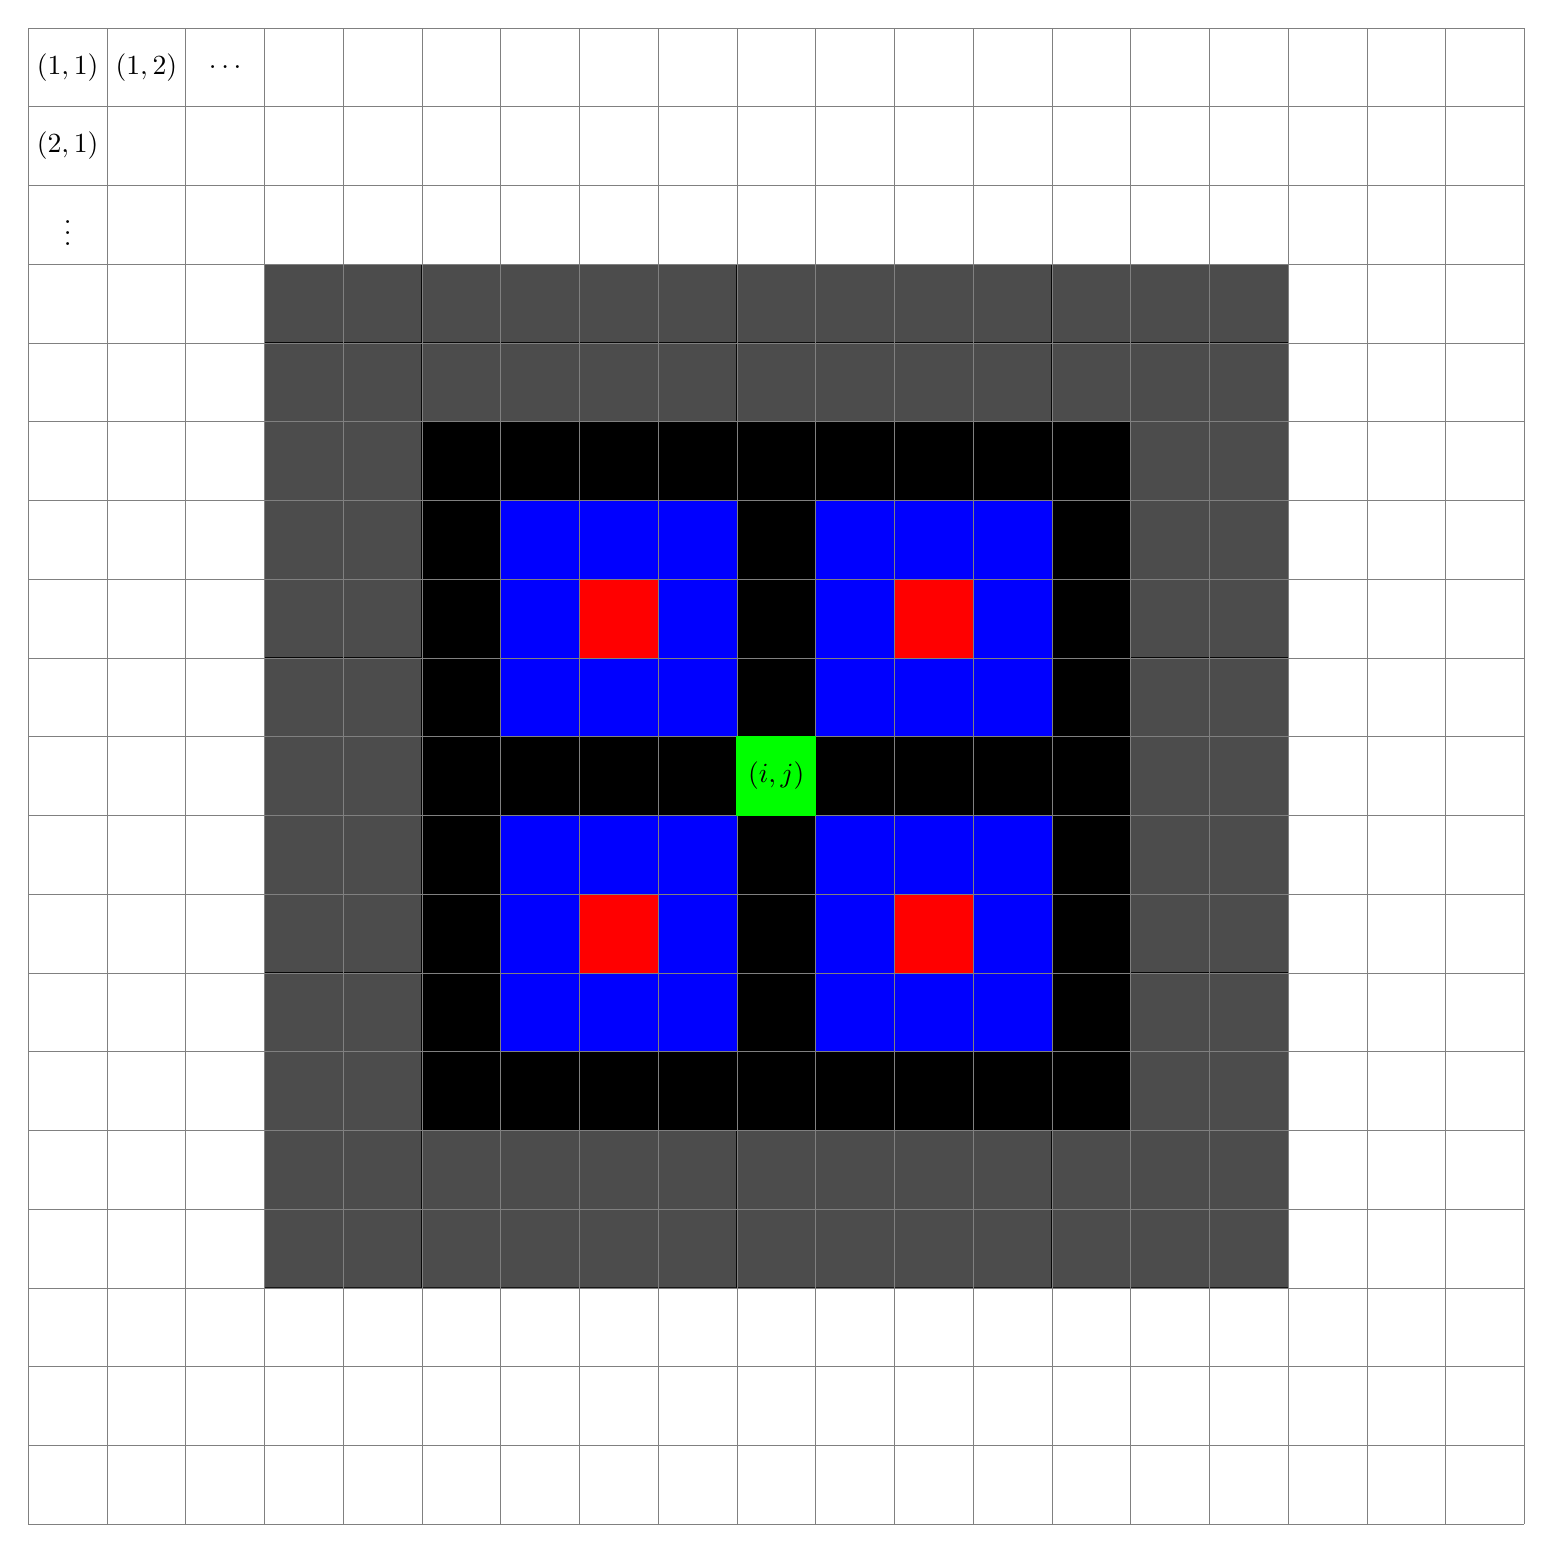
\begin{tikzpicture}
			\foreach \i in {-6, ..., 6}
				\foreach \j in {-6, ..., 6}
					\filldraw[black, opacity=0.7] (\i, \j) rectangle + (1, 1);
			\foreach \i in {-4, ..., 4}
				\foreach \j in {-4, ..., 4}
					\filldraw[black] (\i, \j) rectangle + (1, 1);
			\foreach \x in {(-3, -3), (-3, 1), (1, -3), (1, 1)}
				\filldraw[blue] \x rectangle + (3, 3);
			\foreach \x in {(-2, -2), (-2, 2), (2, -2), (2, 2)}
				\filldraw[red] \x rectangle + (1, 1);
			\draw[help lines, step=1] (-9, -9) grid (10, 10);
			\filldraw[green] (0, 0) rectangle + (1, 1);
			\node at (0.5, 0.5) {$(i, j)$};
			\node at (-8.5, 9.5) {$(1, 1)$};
			\node at (-7.5, 9.5) {$(1, 2)$};
			\node at (-6.5, 9.5) {$\dots$};
			\node at (-8.5, 8.5) {$(2, 1)$};
			\node at (-8.5, 7.5) {$\vdots$};
		\end{tikzpicture}
	}
	\caption{The black area are the pixels that contribute to $(\mathfrak{I} \circ \Psi_\varphi) \bullet \Psi_\varphi)(i, j)$. The blue squares are mutually independent. The red pixels are the pixels that we reduce the intersection in the proof to.}
	\label{fig: powerindependentpoints}
\end{figure}